\documentclass[border=5pt]{standalone}
\usepackage{amsmath,amssymb,mathtools}
\usepackage{tikz}
\usepackage{pgfplots}
\usepackage{pgf}
\begin{document}
	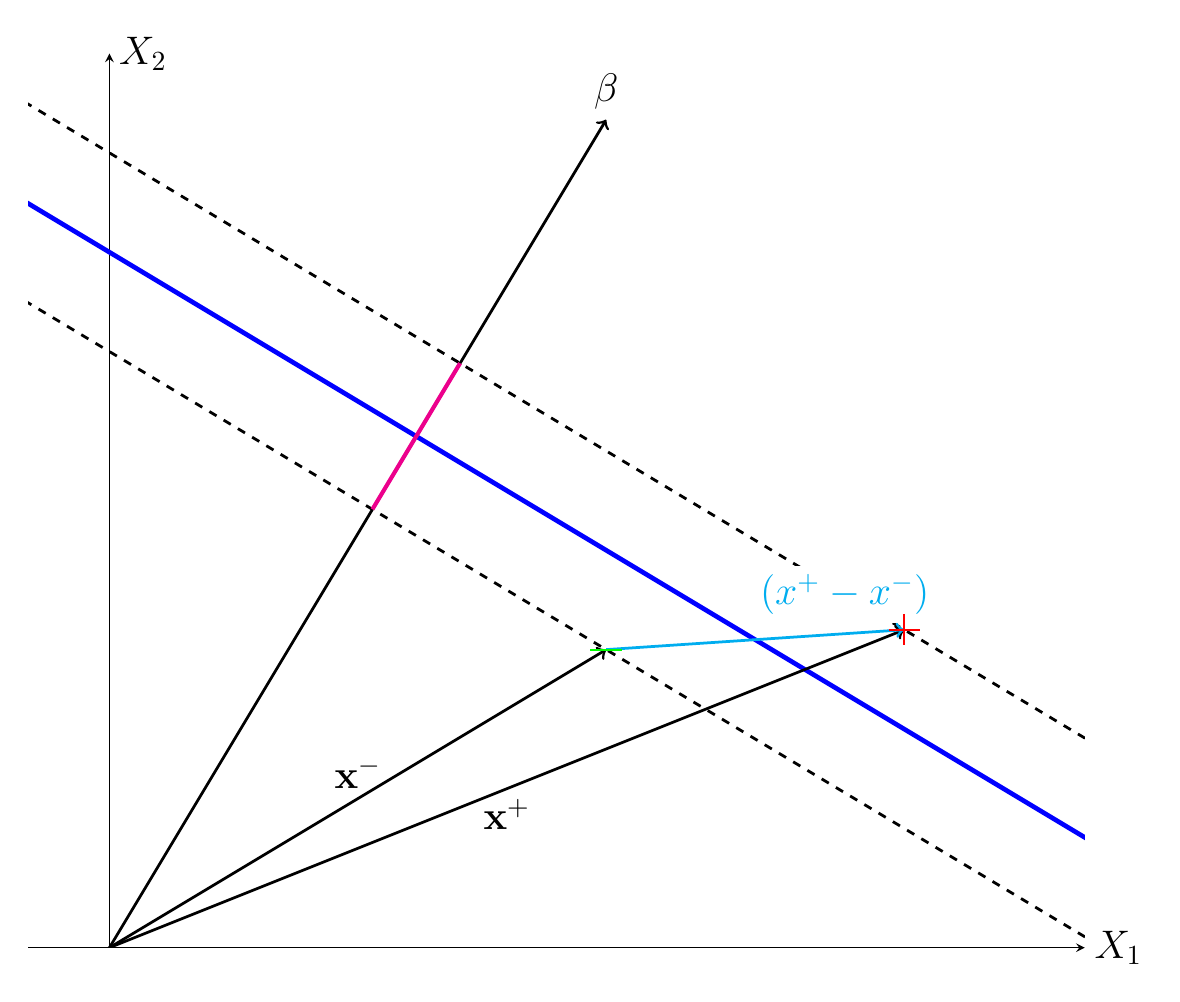
\begin{tikzpicture}
		\begin{axis}[
			xmin=0,
			xmax=9,
			ymin=0,
			ymax=9,
			axis equal,
			axis x line=center,
			axis y line=center,
			xmajorticks=false,
			ymajorticks=false,
			width=15cm,
			ylabel style={right,font=\Large},
			ylabel=$X_2$,
			xlabel style={above,right,font=\Large},
			xlabel=$X_1$
			]
			%\addplot[no markers, domain=-1:11]{(5/3)*x};
			
			\addplot[only marks, mark=-,draw=green,mark size=0.2cm,thick]coordinates {(5,3)};
			\addplot[only marks, mark=+,draw=red,mark size=0.2cm,thick]coordinates {(8,3.2)};
			\addplot[no markers,domain=-1:11,thick,blue,line width=1.7pt]{-0.6*x+7};
			\addplot[no markers, domain=-1:11,dashed,line width=1pt]{-0.6*x+8};
			\addplot[no markers, domain=-1:11,dashed,line width=1pt]{-0.6*x+6};
			
			\draw[->,line width=1pt] (axis cs:0,0)--(axis cs:5,3) node[above,pos=0.5, font=\Large]{$\mathbf{x^-}$};
			\draw[->,line width=1pt] (axis cs:0,0)--(axis cs:8,3.2) node[below,pos=0.5, font=\Large]{$\mathbf{x^+}$};
			\draw[->,line width=1pt] (axis cs:0,0)--(axis cs:5,8.333) node[above,pos=1, font=\Large]{$\beta$};
			\draw[->,cyan,line width=1pt] (axis cs:5,3)--(axis cs:8,3.2) node[above,pos=0.8, font=\Large]{\colorbox{white}{\textcolor{cyan}{$(x^+-x^-)$}}};
			\draw[magenta,thick,line width=1.5pt] (axis cs:2.647058,4.411763)--(axis cs:3.529411,5.882352);
		\end{axis}
	\end{tikzpicture}
\end{document}